\documentclass{beamer}
\usepackage{amsmath}%
\usepackage{amsfonts}%
\usepackage{amssymb}%

%\usepackage{hyperref}

\usepackage{graphicx}
\usepackage{subfig}

\usepackage[czech]{babel}
\usepackage[utf8]{inputenc}

\usepackage{multicol}
%\usepackage{natbib}%
\usepackage{units}

\usepackage{stmaryrd}
\usepackage{gensymb}
\usepackage{bibentry}
\usepackage{accents}

%\usepackage{booktabs}

\usepackage{tensor}
\usepackage[bbgreekl]{mathbbol}
\usepackage{bm}
\usepackage{ulem}

% FANCY TABLES
\usepackage{booktabs}
\usepackage{multirow}
\usepackage{threeparttable}

%\usetheme{Luebeck}
%\usetheme{Madrid}
\usetheme{CambridgeUS}
%\usetheme{Pittsburgh}
%\usetheme{default}
%\mode<presentation>

%FOR CAMBRIDGE US THEME -- red bullets/captions in itemize environment
\setbeamercolor{item projected}{bg=red}
\setbeamertemplate{enumerate items}[default]
\setbeamertemplate{navigation symbols}{}
\setbeamercovered{transparent}

\setbeamercolor*{enumerate item}{fg=red}
\setbeamercolor*{enumerate subitem}{fg=red}
\setbeamercolor*{enumerate subsubitem}{fg=red}

\setbeamercolor{block title}{fg=red}
\setbeamercolor{caption name}{fg=red}

\uselanguage{Czech}
\languagepath{Czech}
\deftranslation[to=Czech]{Theorem}{Věta}
\newtheorem{exercise}[theorem]{Příklad}

\usepackage{listings,xcolor}

\title[Přerovnání řad]{Přerovnání neabsolutně konvergentních řad}
\author{Petr Rašek, Matúš Letko}
\institute[Charles University]{Charles University, Czech Republic}
\date{\today}


\let\newblock\relax

\begin{document}

\begin{frame}
\titlepage
\bibliographystyle{plain}
\end{frame}

\section{Teorie}
\label{sec:introduction}


\begin{frame}
  \frametitle{Teorie}
  \begin{Definition}[Přerovnání řady]
  Nechť \{\(a_n\} \subset \mathbb{R}\) a \(\varphi : \mathbb{N} \rightarrow \mathbb{N}\) je bijekce. Pak řadu 
  \(\sum _{n=1} ^{\infty} a_{\varphi(n)}\) nazveme \textit{přerovnáním} řady \(\sum _{n=1} ^{\infty} a_n\) (odpovídajícím bijekci \(\varphi\)).
  \end{Definition}
  \begin{Theorem}[Riemannova] 
  \normalfont Nechť \{\(a_n\} \subset \mathbb{R}\) a řada \(\sum _{n=1} ^{\infty} a_n\) konverguje neabsolutně. Pak pro každé \(S \in \mathbb{R} ^\ast\) existuje přerovnání řady \(\sum _{n=1} ^{\infty} a_n\) se součtem \(S\)
  \end{Theorem}
  \begin{exercise}[Neabsolutně konvergentní řady]
    \begin{itemize}
        \item \(\sum _{n=1} ^{\infty} \frac{(-1)^{n+1}}{n} = \log(2)\)
        \item \(\sum _{n=2} ^{\infty} \frac{(-1)^{n}}{n\log(n)} = 0.526412\)
        \item \(\sum _{n=1} ^{\infty} \frac{\sin(n)}{n} = \frac{1}{2}(\pi - 1)\)
    \end{itemize}
  \end{exercise}
\end{frame}

\section{Ilustrace}
\begin{frame}
  \frametitle{\(\sum _{n=1} ^{\infty} \frac{(-1)^{n+1}}{n}\)}
  Cílový součet 1
  \begin{center}
    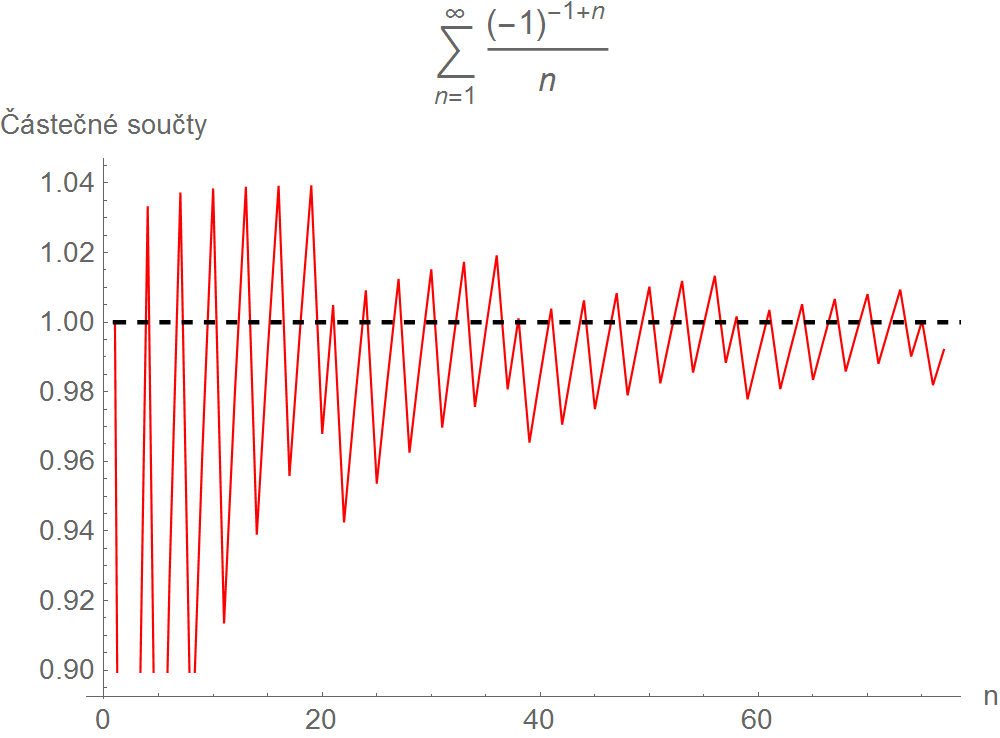
\includegraphics[width=0.8\textwidth]{serie1_1.png}
  \end{center}
\end{frame}

\begin{frame}
  \frametitle{\(\sum _{n=1} ^{\infty} \frac{(-1)^{n+1}}{n}\)}
  Cílový součet 2
  \begin{center}
    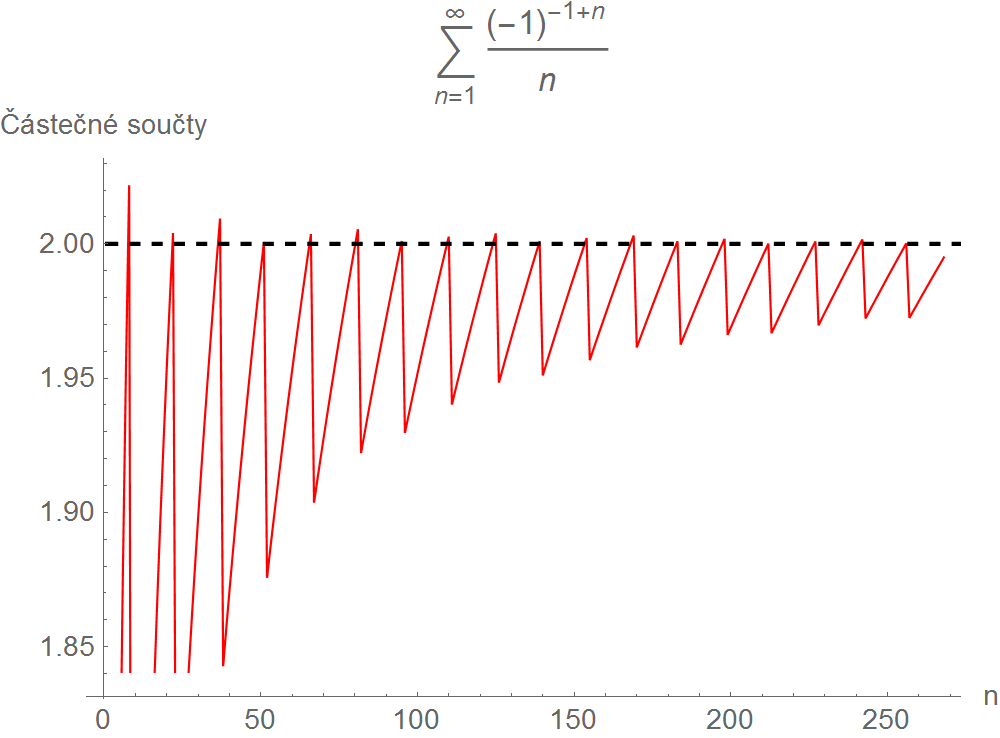
\includegraphics[width=0.8\textwidth]{serie1_2.png}
  \end{center}
\end{frame}

\begin{frame}
  \frametitle{\(\sum _{n=1} ^{\infty} \frac{(-1)^{n+1}}{n}\)}
  Cílový součet \(\ -\frac{1}{2}\)
  \begin{center}
    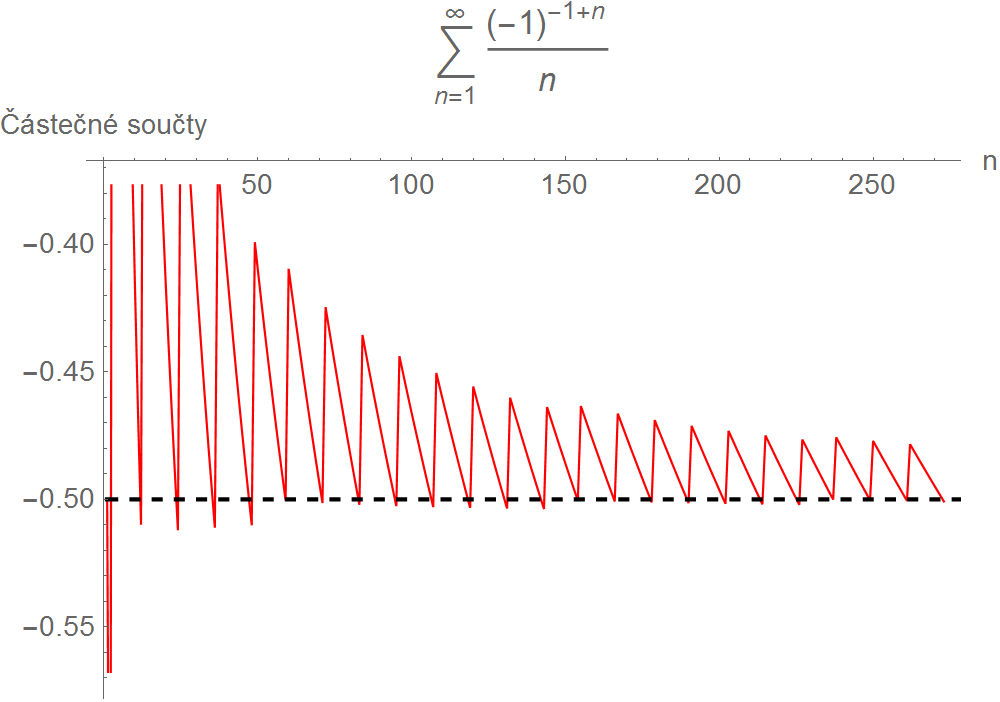
\includegraphics[width=0.8\textwidth]{serie1_3.png}
  \end{center}
\end{frame}

\begin{frame}
  \frametitle{\(\sum _{n=2} ^{\infty} \frac{(-1)^{n}}{n\log(n)}\)}
  Cílový součet \(\frac{1}{2}\)
  \begin{center}
    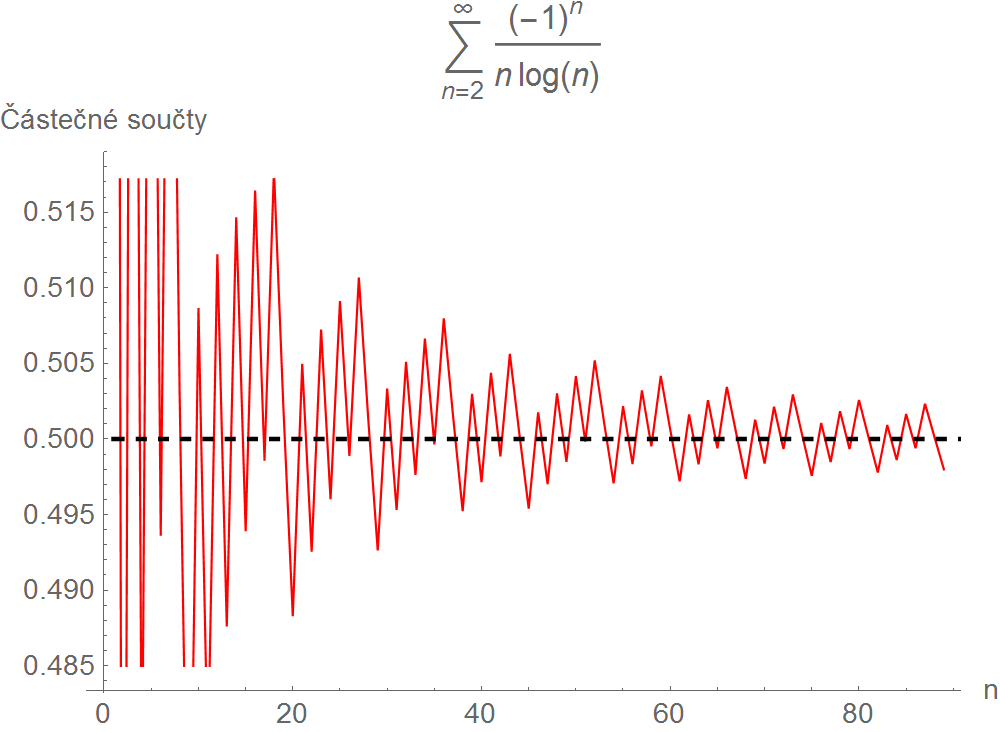
\includegraphics[width=0.8\textwidth]{serie2_1.png}
  \end{center}
\end{frame}

\begin{frame}
  \frametitle{\(\sum _{n=2} ^{\infty} \frac{(-1)^{n}}{n\log(n)}\)}
  Cílový součet 1
  \begin{center}
    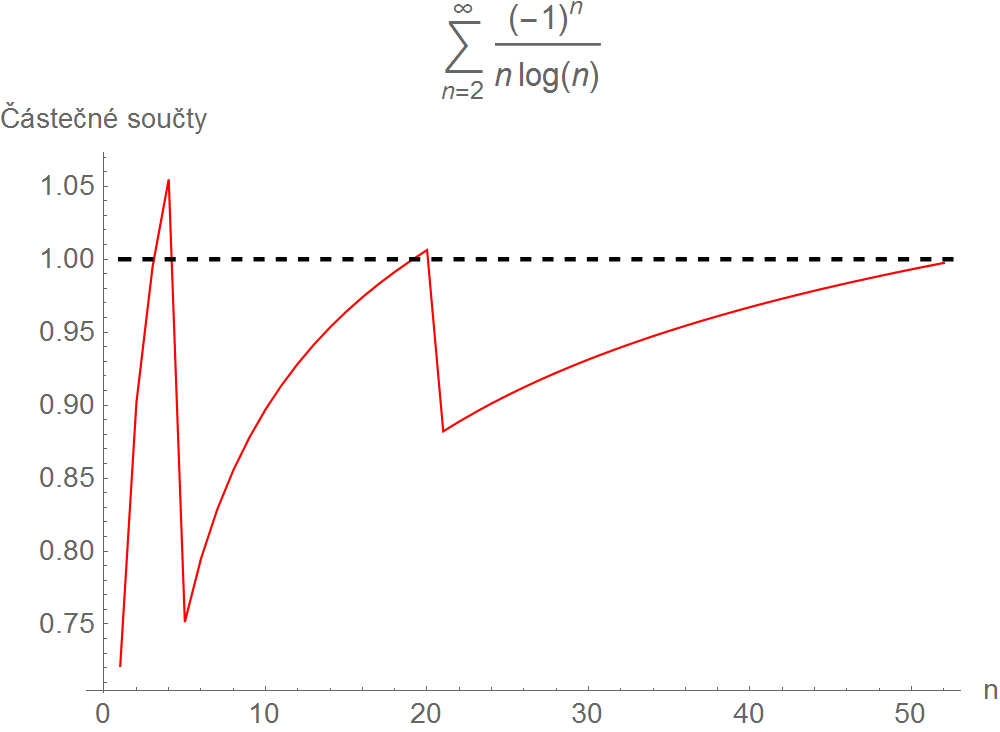
\includegraphics[width=0.8\textwidth]{serie2_2.png}
  \end{center}
\end{frame}

\begin{frame}
  \frametitle{\(\sum _{n=1} ^{\infty} \frac{\sin(n)}{n}\)}
  Cílový součet 1
  \begin{center}
    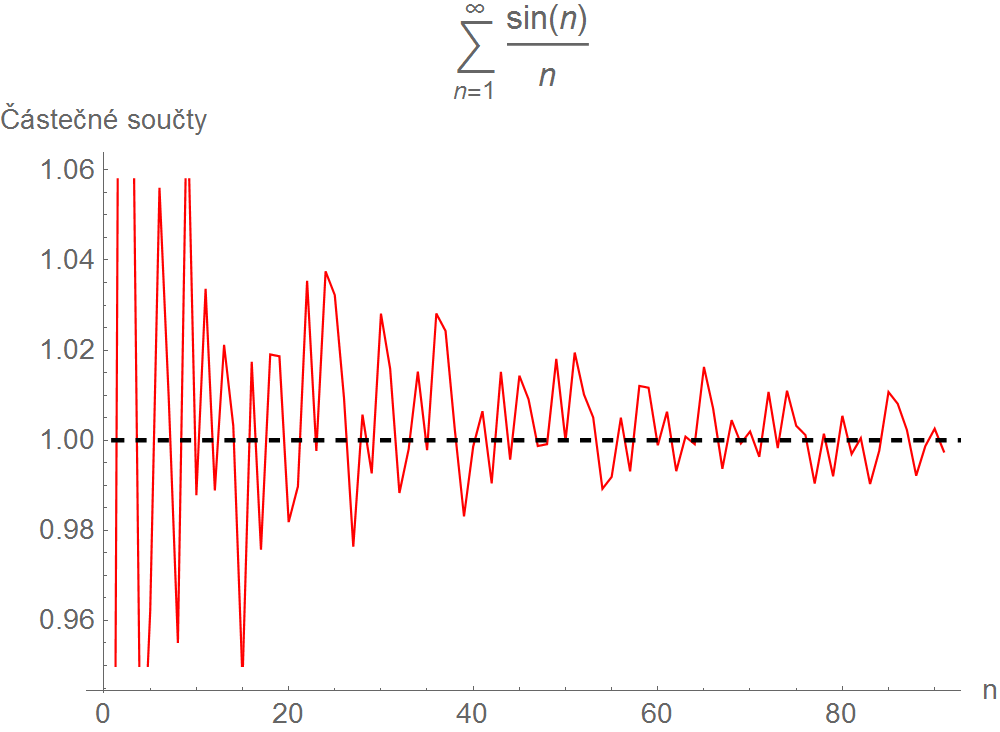
\includegraphics[width=0.8\textwidth]{serie3_1.png}
  \end{center}
\end{frame}

\begin{frame}
  \frametitle{\(\sum _{n=1} ^{\infty} \frac{\sin(n)}{n}\)}
  Cílový součet 3
  \begin{center}
    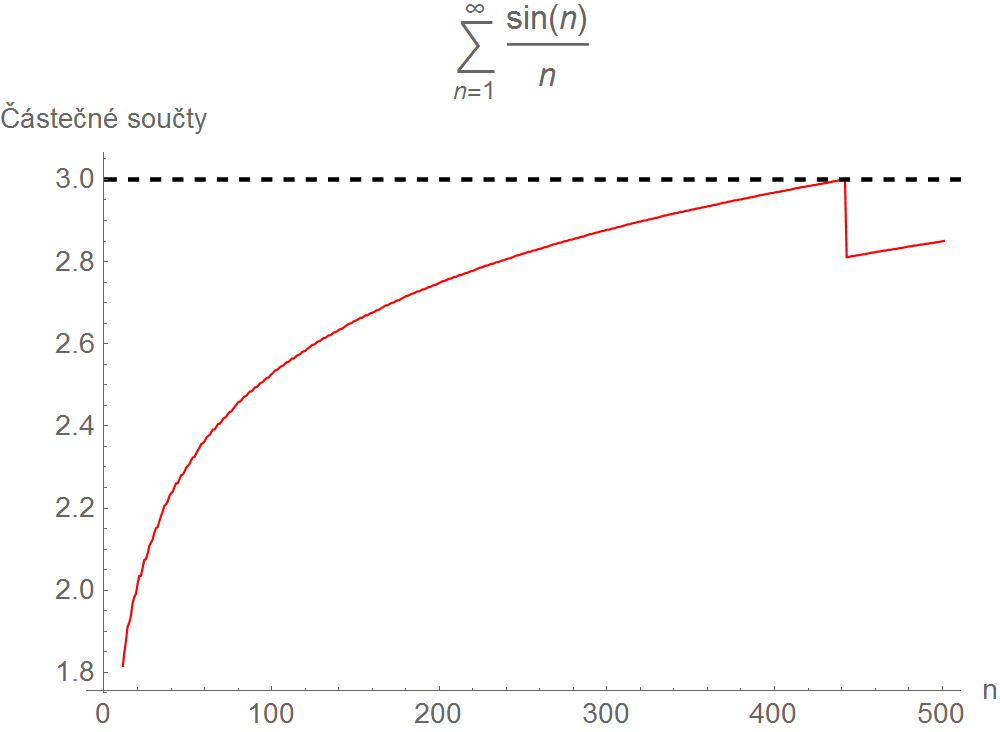
\includegraphics[width=0.8\textwidth]{serie3_2.png}
  \end{center}
\end{frame}

\end{document}

%
%
%
%
% DOCUMENT ENDS HERE
%
%
%
%




